\chapter{Metodologia}
\label{chap:metodologia}

\section{Descrição de Sistemas de Abastecimento de Água}

Os sistemas de abastecimento de água são projetados para fornecer água potável às populações urbanas e rurais. São essenciais para a saúde pública, a economia e o bem-estar geral das comunidades. A descrição a seguir detalha os componentes e operações típicas de um sistema de abastecimento de água.

\subsection*{Fontes de Abastecimento}

A escolha do tipo de fonte de água é influenciada por diversos fatores, incluindo a disponibilidade e qualidade da água, o custo de tratamento e condições locais específicas. As fontes podem ser classificadas em duas categorias principais: superficiais e subterrâneas. As fontes superficiais incluem rios, lagos e represas, enquanto as fontes subterrâneas abrangem aquelas provenientes de poços artesianos ou poços tubulares profundos.

\subsection*{Componentes do Sistema de Abastecimento de Água}


\begin{itemize}
\item[] Bomba de Água:
\item[-] Centrífugas monoestágio: Estas bombas possuem apenas um estágio de bombeamento, ou seja, um conjunto de rotor e difusor que gera a pressão e a vazão do líquido. São indicadas para casos onde se necessita de uma alta vazão e uma baixa pressão, como em indústrias e abastecimentos de pequenos prédios. 

\item[-] Autoaspirantes: Possuem um sistema que permite que elas retenham a água no corpo da bomba, facilitando o seu funcionamento. São indicadas para casos onde a altura de sucção é superior a 8 metros e não é possível fazer a instalação de uma válvula de pé na extremidade do tubo de sucção. 

\item[-] Multiestágios horizontal ou vertical: Possuem vários estágios de bombeamento, ou seja, vários conjuntos de rotores e difusores que geram a pressão e a vazão da água. São indicadas para casos onde se necessita de uma alta vazão e uma alta pressão, como em sistemas de abastecimento público ou industrial. 

\item[-] Periféricas: Possuem um rotor com palhetas radiais, que criam uma zona de baixa pressão na entrada da bomba e uma zona de alta pressão na saída da bomba. São indicadas para casos onde se necessita de uma baixa vazão e uma alta pressão, como em sistemas de irrigação. 

\item[-] Submersas: Funcionam dentro da água, em contato com o líquido. São indicadas para poços profundos e aplicações onde a bomba precisa ser submersa no líquido que está sendo bombeado. 
\end{itemize}
    
A seleção adequada da bomba é crucial para garantir que o sistema de abastecimento opere de maneira eficiente, minimizando os custos operacionais e garantindo a entrega de água de qualidade aos consumidores. A escolha da bomba deve considerar fatores como a vazão necessária, a altura manométrica, a eficiência energética, entre outros. 

Neste trabalho consideramos uma bomba genérica, hipotética, com consumo de 1 kW e vazão de saída de 2 m³/h. Esses valores foram baseados em bombas amplamente utilizadas no mercado, tomando como referência o modelo Schneider BC-21 R 1 1/4 de 1,5 cv. É uma bomba centrífuga monoestágio que pode ser usada para irrigação, abastecimento predial, sistemas de refrigeração, fontes e cascatas, entre outras aplicações industriais. Possui potência de 1,1 kW e vazão máxima de 18,2 m³/h \cite{Schneider}.

\begin{figure}[h]
    \centering
    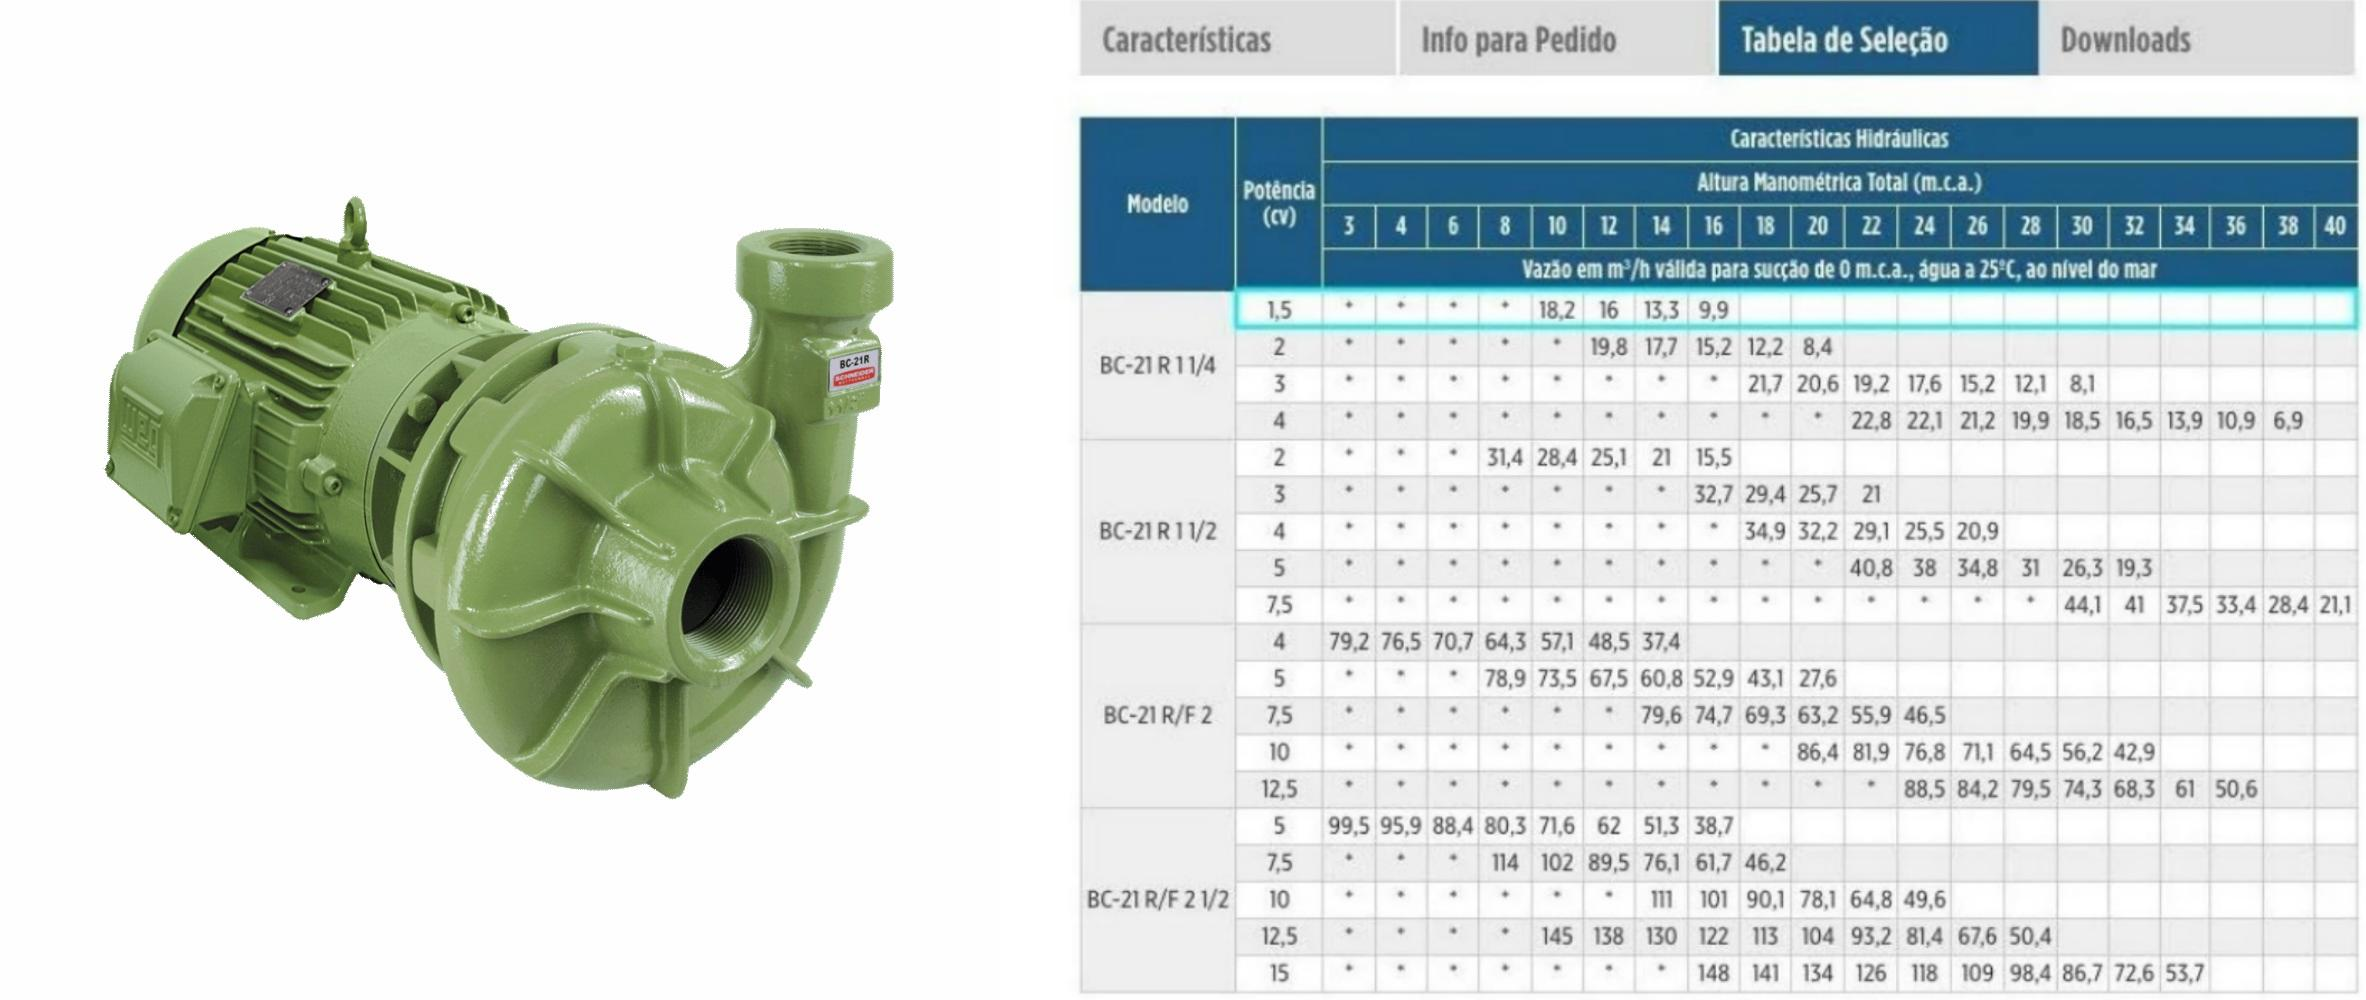
\includegraphics[scale=0.8]{figuras/1111111111111111111111111.jpg}
    \caption{Bomba Modelo - Schneider BC-21 R 1 1/4}
        \label{fig:1}
\end{figure}

\textit{Reservatórios:}

São estruturas que armazenam água para garantir o fornecimento contínuo, mesmo durante períodos de alta demanda ou quando a fonte de água não estiver disponível. Sua capacidade depende da vazão da bomba e da demanda de consumo.

Existem dois tipos principais dessas estruturas. Os reservatórios elevados são geralmente feitos de concreto ou aço e estão elevados do solo para fornecer pressão por gravidade. Já os reservatórios apoiados estão localizados no nível do solo ou enterrados, e requerem bombeamento ou sistemas de pressão para distribuir a água.


No projeto em questão, foi adotado um modelo de reservatório elevado com capacidade máxima de 20 m³. Este modelo foi escolhido por fornecer abastecimento por gravidade, eliminando os gastos com distribuição de água.

\textit{Rede de Distribuição:}

É o sistema de tubulações que transporta a água dos reservatórios até os consumidores. Ela é composta por tubulações principais, secundárias e ramais. A manutenção regular desta rede é crucial para prevenir vazamentos e garantir a qualidade da água.

    
\section{Tarifação e Políticas de Consumo}

A tarifação e as políticas de consumo desempenham um papel decisivo na gestão eficiente dos sistemas de abastecimento de água. São instrumentos que influenciam o comportamento do consumidor e a operação do sistema, visando alcançar objetivos específicos, como a sustentabilidade financeira, a equidade no acesso e o uso racional da água \cite{sancho19WaterConsumption}. 

\subsection*{Tarifação}   

As tarifas podem ser estruturadas de diversas formas, dependendo dos objetivos a serem alcançados, tais como: 

\begin{itemize}

    \item[-] Tarifas Fixas: Um valor fixo é cobrado, independentemente do volume de água consumido. Este tipo de tarifa é simples, mas não incentiva o uso eficiente da água. 

    \item[-] Tarifas Variáveis: A tarifa é baseada no volume de água consumido. Pode ser uma taxa uniforme por unidade de volume ou pode variar de acordo com faixas de consumo, incentivando a economia de água. 

    \item[-] Tarifas Diferenciadas por Horário: As tarifas variam de acordo com o horário do dia, refletindo os custos variáveis de fornecimento. Por exemplo, tarifas mais altas podem ser aplicadas durante os horários de pico, para desencorajar o uso excessivo e aliviar a pressão sobre o sistema.

\end{itemize}


Esquemas tarifários são uma ótima alternativa para a otimização do consumo de energia, pois permitem que decisões sejam tomadas com base nos custos associados a cada tarifa. Por exemplo, pode ser mais econômico operar equipamentos que consomem muita energia durante os períodos em que a tarifa mais barata é aplicada ou evitar consumos excessivos em horários de alta tarifa. 


\subsection{Políticas de Consumo}

Além da tarifação, políticas de utilização podem ser implementadas para gerenciar o consumo de água: 

\begin{itemize}

\item[-] Restrições de Uso: Em situações de escassez, podem ser impostas restrições sobre certos usos não essenciais da água, como rega de jardins ou lavagem de carros. 

\item[-] Programas de Educação: Campanhas de conscientização podem ser lançadas para informar e alertar a população sobre a importância do consumo sustentável de água e energia.

\item[-] Incentivos: Incentivos podem ser oferecidos à população para encorajar práticas de economia de água, como a instalação de dispositivos de baixo fluxo ou a coleta de água da chuva. 

\end{itemize}

No trabalho, foi observado que a tarifação desempenha um papel significativo na otimização do custo de energia associado ao abastecimento de água. Elas são diferenciadas por períodos tarifários, e a operação da bomba é ajustada de acordo com essas tarifas para minimizar os custos. Além disso, políticas fixas com restrições de tarifa de ponta são implementadas para otimizar ainda mais o funcionamento da bomba e os custos associados. 

Essa combinação proporcionou uma otimização no consumo, que pode incentivar uma gestão mais eficiente dos recursos energéticos, beneficiando tanto os prestadores de serviços quanto os consumidores. 

\section{Análise e Visualização dos Dados}
  

\section{Modelagem Matemática}

O problema consistia em determinar o melhor momento para ligar e desligar uma bomba de água, responsável pelo abastecimento de um reservatório, de forma a minimizar os custos com energia elétrica associados, mantendo o nível de água armazenada dentro de limites aceitáveis.

Os custos variam conforme uma tarifa, que muda ao longo do dia e da semana, enquanto o nível do reservatório é determinado pela vazão da bomba, pela demanda de consumo e pela capacidade do próprio reservatório.

O modelo foi formulado como um problema de programação linear inteira mista, usando variáveis binárias para representar o estado da bomba (ligada ou desligada) e variáveis contínuas para representar os níveis do reservatório.

A função objetivo foi projetada para minimizar o custo total com energia elétrica ao longo do horizonte de planejamento de uma semana, sujeita a restrições que incluíam o balanço de massa do reservatório, os limites do nível do reservatório e a relação entre o estado e a vazão da bomba.

\subsection{Formulação matemática}


\subsection{Conjuntos e parâmetros}

\begin{itemize}

\item[-] $h = \left\{1, ..., 24\right\}$: conjunto das horas do dia.

\item[-] $d = \left\{1, ..., 7\right\}$: conjunto dos dias da semana.

\item[-] $C_{h,d}$: custo da energia elétrica na hora $h$ e no dia $d$ ($R\$/kWh$).

\item[-] $P$: potência da bomba ($kW$).

\item[-] $Q$: vazão da bomba ($m^3/h$).

\item[-] $V_{min}$: limite mínimo do nível do reservatório ($m^3$).

\item[-] $V_{max}$: limite máximo do nível do reservatório ($m^3$).

\item[-] $V_{0}$: nível inicial do reservatório ($m^3$).

\item[-] $D_{h,d}$: demanda de consumo na hora $h$ e no dia $d$ ($m^3/h$).

\end{itemize}


\subsection{Variáveis de decisão}

\begin{itemize}

\item[-] $x_{h,d} \in {0, 1}$: variável binária que indica se a bomba está ligada (1) ou desligada (0) na hora h e no dia d.

\item[-] $V_{h,d} \geq 0$: variável contínua que representa o nível do reservatório na hora h e no dia d ($m^3$).
\end{itemize}

\subsection{Função objetivo}

O objetivo é minimizar o custo total com energia elétrica ao longo do horizonte de planejamento, dado por:

$$min \sum_{h=1}^{24} \sum_{d=1}^{7} C_{h,d} P x_{h,d}$$

\subsection{Restrições}

Balanço de massa do reservatório:

\BlankLine

$V_{h,d} = V_{h-1,d} + Q x_{h,d} - D_{h,d}, \forall h \in {2, ..., 24}, \forall d \in D$

$V_{1,d} = V_{24,d-1} + Q x_{1,d} - D_{1,d}, \forall d \in {2, ..., 7}$

$V_{1,1} = V_0 + Q x_{1,1} - D_{1,1}$

\BlankLine

Limites do nível do reservatório:

\BlankLine

 $V_{min} \leq V_{h,d} \leq V_{max}, \forall h \in H, \forall d \in D$


\section{Otimização do Problema}

A otimização da gestão em sistemas de abastecimento de água constitui um desafio multidimensional, que envolve a sincronização entre demanda, oferta e custos operacionais. No presente estudo, abordamos a otimização do funcionamento de bombas de água em um sistema de abastecimento, focando no equilíbrio entre a demanda horária de consumo de água e as variações tarifárias de energia elétrica, com o intuito de minimizar o custo energético sem comprometer a disponibilidade hídrica para os consumidores.

A análise foi iniciada com a criação de uma matriz de demanda horária média, de consumo de água para cada dia da semana, baseada em registros históricos. Cada célula da matriz 
Para a otimização, foram definidos parâmetros críticos, como a potência da bomba, a taxa de fluxo de água e a capacidade do reservatório. O volume inicial do reservatório foi estabelecido, assim como os volumes mínimo e máximo, para assegurar uma operação dentro dos limites seguros e eficientes.


\subsection{Estratégia de Tarifação Dinâmica}

A estratégia de tarifação dinâmica foi implementada considerando três tarifas distintas, baseadas na bandeira verde: a tarifa vermelha, para horários de pico; a tarifa amarela, para horários intermediários; e a tarifa verde, para horários de baixa demanda. A função de precificação foi configurada para atribuir a tarifa correspondente a cada intervalo horário, com diferenciação entre dias úteis e fins de semana.


\subsection{Algoritmo de Simulação de Operação das Bombas}


\subsection{Monitoramento e Restrições de Operação}

As restrições de operação, como níveis críticos do reservatório e a capacidade máxima de bombeamento, foram rigorosamente monitoradas, e qualquer violação das restrições foi registrada para posterior análise e ajuste da estratégia de operação.


Visualizações gráficas foram criadas para ilustrar o consumo de água por hora e dia da semana, o nível do reservatório ao longo do tempo, o custo acumulado da energia elétrica e a distribuição temporal da operação das bombas em relação às tarifas aplicadas. Essas visualizações foram fundamentais para identificar padrões de consumo, avaliar a eficácia das estratégias de operação e compreender o impacto das tarifas na operação do sistema.



\subsection{Conclusão}

Ao final do processo de otimização, observou-se uma redução significativa nos custos com energia elétrica, indicando a eficiência das estratégias de operação adotadas. Com a primeira política de funcionamento, sem restrição de funcionamento em horários de pico, o consumo semanal foi de R\$ 12,97, enquanto que com a política proposta, restritiva quanto ao funcionamento das bombas em horário de pico o custo foi de R\$ 8,71, uma economia de 32.85\%.

Portanto, a abordagem implementada demonstrou ser uma solução viável para a gestão sustentável de sistemas de abastecimento de água, equilibrando custos operacionais e disponibilidade hídrica.
